\chapter{Introduction to quantum geometry}
\label{chap:driving}
This chapter depends on the mathematical formalism developed in Chapter \ref{chap:mathIntro}, and some basic knowledge of quantum mechanics is required. Most parts are inspired by notes by \citet{kolodrubez} and original notes by \citet{berry1984}(1984), \cite{berry1989}(1989), \cite{berry2009}(2009) with attempt to give them more rigorous meaning in the language of differential geometry. 

The aim of this chapter is the construction of space on which the \emph{driving of quantum states} (changing the states by controlling the Hamiltonian parameter) is performed and introducing some basic concepts needed. There may be many geometrical constructions of the space because usually, only some sections of the full space are used. Different constructions require different mathematical formalism. One might choose the way of \emph{vector bundles}, or \emph{fiber bundles} (our case), or just sectioning one Hilbert space in different ways, constructing the needed physical spaces. The reason for choosing the way of fiber bundles is that from the Hamiltonian with free parameter $\HH(\lambda)$, we get one Hilbert space for every parameter value. The fiber structure then gives the natural formalism for connecting these spaces and embeds the space with natural geometry due to changing eigenbasis during the driving. In addition, the fiber space holds the information about driving parameter $\lambda$.

Even though the theory below depends on differential geometry, it does not reformulate the whole quantum mechanics into this language. This kind of reformulation is a rather complicated task and for an introduction to this approach, see Appendix \ref{appendixGEOM}.

From now on, we use natural units, so $\hbar=1$.

\section{Space of all states}
Assume parameter $\llambda\in\mathcal{U}\subset\R^N$ for $\mathcal U$ open set. This parameter controls some finite-dimensional Hamiltonian $\HH(\llambda)$, which is bounded from below and has discrete spectrum. From this we can construct the fiber bundle, such that at every point of the base manifold $\llambda\in \mathcal{U}$, we construct fiber as a Hilbert space $\H(\llambda)$. The fiber structure can be according to Def. \ref{def:fiberBundle} written as
$$\left(\H_{full}\coloneqq \bigcup_{\llambda\in\mathcal U} \H(\llambda),\;\;\mathcal{U}\subset \R^N,\;\;\pi,\;\; \H(\llambda) \coloneqq \bigcup_{states}\ket{\psi(\llambda)}  \right).$$
The projection is defined as $\pi(\llambda): \ket{\psi(\llambda)}\mapsto \llambda$ and $\H(\llambda)$ is a Hilbert space containing all pure states of $\HH(\llambda)$. Geometric intuition is displayed in Fig. \ref{fig:wholeBundle}.

\begin{figure}[H]
    \centering
    % 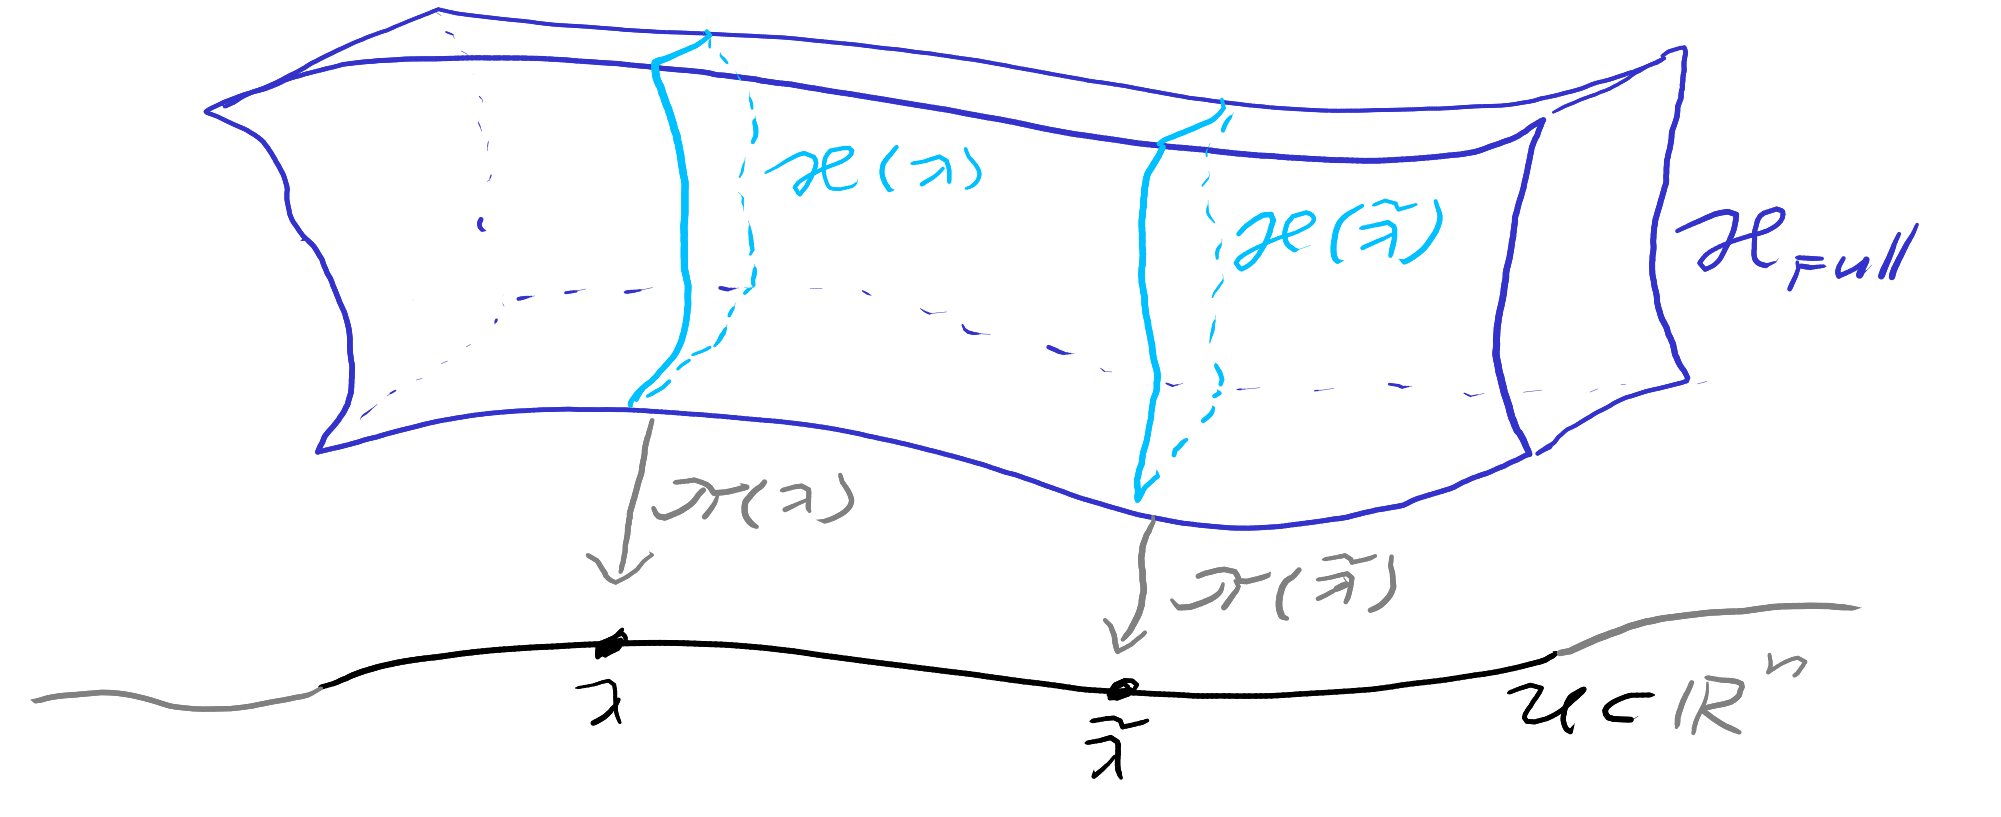
\includegraphics[width=\textwidth]{../img/manifold_basic_1.png}
    \begin{tikzpicture}
        \node[] at (0,0) {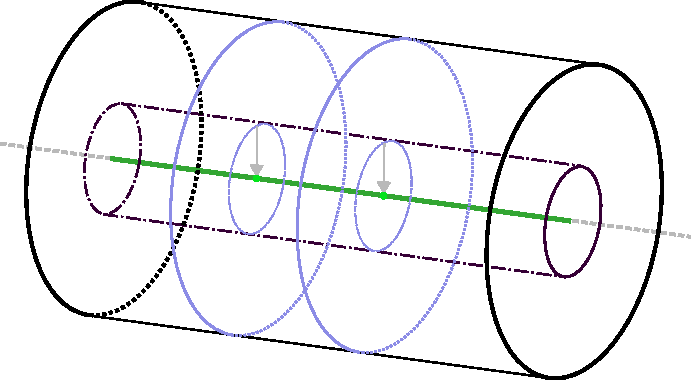
\includegraphics[width=0.7\textwidth]{../img/fullHilbert.pdf}};
        \node[] at (3.4,-0.2) {$\greenn{\mathcal U}$};
        \node[] at (5.6,-0.7) {$\gray{\R^N}$};
        \node[] at (4.6,1.8) {$\H_{full}$};
        \node[] at (-1.0,2.7) {$\blueee{\H(\llambda)}$};
        \node[] at (1.0,2.5) {$\blueee{\H(\tilde\llambda)}$};
        \node[] at (-0.8,0.55) {$\gray{\pi(\llambda)}$};
        \node[] at (1.05,0.3) {$\gray{\pi(\tilde\llambda)}$};
        \node[] at (-1.4,-0.17) {\green{$\llambda$}};
        \node[] at (0.5,-0.4) {\green{$\tilde\llambda$}};
    \end{tikzpicture}

\caption{Base manifold $\greenn{\mathcal U}\subset \gray{\R^N}$ is visualized as a line. For every point $\green\llambda\in\greenn{\mathcal U}$ one \bluee{Hilbert space $\H(\llambda)$ (blue disk)} is constructed as a \bluee{fiber}. The union of all these fibers creates the full Hilbert space $\H_{full}$ (holow cylinder) and from every Hilbert space there exist projection $\gray{\pi}$ onto the base manifold.}
    \label{fig:wholeBundle}
\end{figure}



\section{Rays and bare states}
Physical observables in quantum mechanics are related to the \emph{space of rays} or \emph{projective Hilbert space}, defined as $\P\H\coloneqq \H/U(1)$, where elements of $U(1)$ are unitary transformations $e^{i\varphi}$ for $\varphi\in[0,\pi)$. This defines the \bluee{global} gauge symmetry between quantum states. The phase $\varphi$ is \bluee{chosen the same for every vector} and can be chosen arbitrarily. We cannot alter the phase of individual vectors, meaning there is no local gauge symmetry. 

This resembles the fiber structure
$$\left(\H,\;\P\H,\;\pi_{rays},\;\{e^{i\varphi}| \varphi\in[0,2\pi)\}\right),$$
where $\pi_{rays}$ is just rule setting phase $\varphi$ to arbitrary value. The geometrical intuition is drawn on Fig. \ref{fig:projectiveHilbertSpace}.



\begin{figure}[H]
    \centering
    % 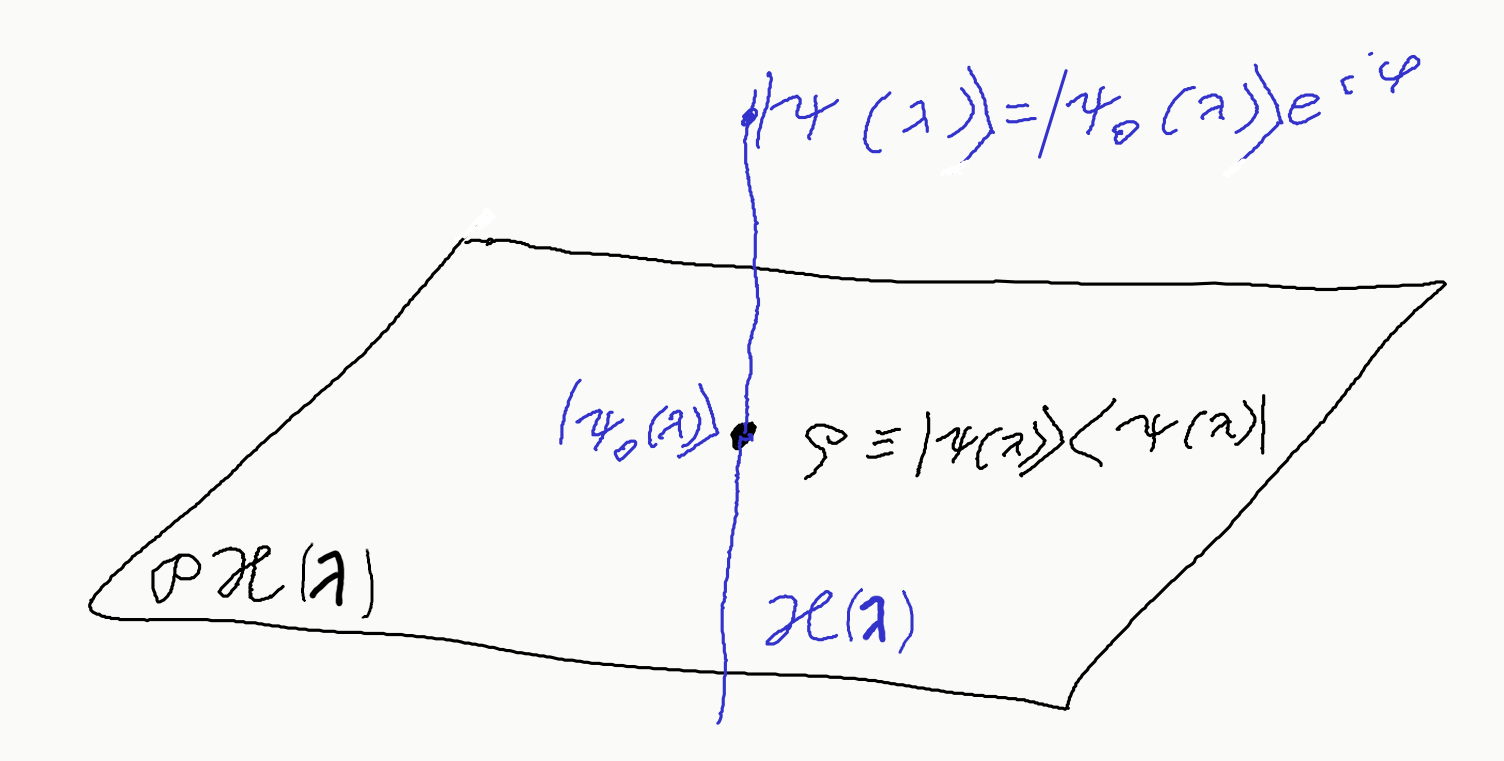
\includegraphics[width=0.8\textwidth]{../img/projectiveHilbertSpace.png}
    \begin{tikzpicture}
        \node[] at (0,0) {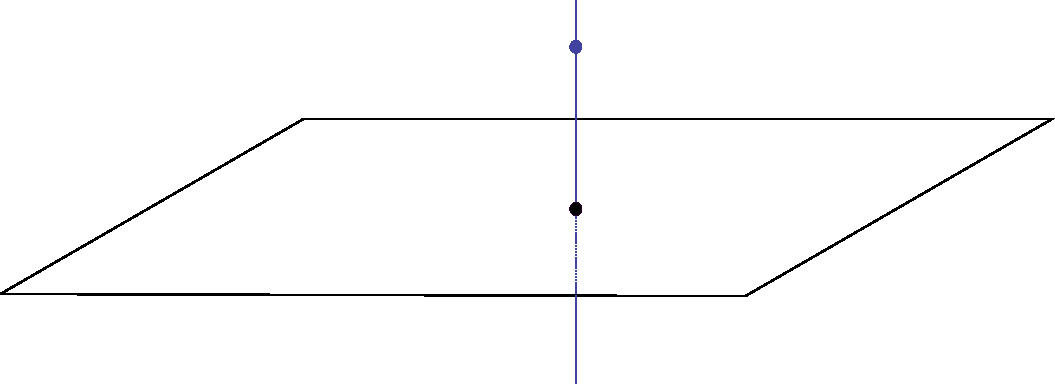
\includegraphics[width=0.7\textwidth]{../img/drawing-projectiveSpace.pdf}};
        \node[] at (3.4,-0.15) {$\bluee{\ket{\psi_0(\llambda)}} \; 
        \leftrightarrow \;\rho\equiv \ket{\psi(\llambda)}\!\!\bra{\psi(\llambda)}$};
        \node[] at (2.6,1.4) {\bluee{$\ket{\psi(\llambda)}=e^{i\varphi}\ket{\psi_0(\llambda)}$}};
        \node[] at (-3,-0.7) {$\P\H(\llambda)$};
    \end{tikzpicture}
\caption{For every $\llambda$ we have the projective Hilbert space $\P\H(\llambda)$ containing physical states $\ket{\psi(\llambda)}$ corresponding to density matrix $\rho\equiv\ket{\psi(\llambda)}\!\!\bra{\psi(\llambda)}$. Every state can be multiplied by phase \bluee{factor $e^{i\varphi}$}, extending it to \bluee{Hilbert space $\H(\llambda)$}.}
    \label{fig:projectiveHilbertSpace}
\end{figure}







\section{Sectioning the space}
Consider initial state $\ket{\psi_0}\in \HH(\llambda_0)$. The state then evolves along some path 
\begin{equation}
    \mathcal J\coloneqq\{\llambda(t)|t\in[0,T],\; \llambda\in \mathcal U\} \subset \R^N,\quad \llambda(0)=\llambda_0
    \label{eq:defJ}    
\end{equation}
parametrized by time $t$, according to the Schr\"odinger equation
\begin{equation}
    i\hbar \der{}{t}\kpsilt = \HH(\llambda(t))\kpsilt.
    \label{eq:schrodinger}
\end{equation}
For eigenstates $\{\ket{s}\}_{s=0}^{N-1}$ of instantaneous Hamiltonian it reads as a Schr\"odinger energy equation
\begin{equation}
    \HH(\llambda)\ket{s(\llambda)}=E_s(\llambda)\ket{s(\llambda)}.
    \label{eq:energySchrodinger}
\end{equation}
Notice that these states are independent on the trajectory $\mathcal J_t$.
For every $\HH(\llambda)$ its energies can be sorted from the smallest, defining the \emph{Hamiltonian spectrum}
\begin{equation}
    \sigma(\HH(\llambda))\coloneqq\{E_0,\dots,E_{N-1}\}.
\end{equation}
In this set degeneracies are not unified into one element, therefore every $\sigma(\llambda)$ has $N$ elements. From this there exists an isomorphism between all $\sigma$-sets, and we can define \emph{section} 
$$\mathrm{sec}_s: \ket{s(\llambda)}\mapsto \mathcal{U}\subset \R^N, \quad \text{for } s\in\{0,\dots, N-1\}.$$
This maps eigenstates corresponding to energy $E_s$ to the base manifold. This mapping is similar to previously introduced $\pi$, except it is an isomorphism, not a projection. The isomorphism is showed later on, when introducing the metric structure on these spaces.

Now we have constructed $N$ sections of the full Hilbert space, which are isomorphic to the base manifold. Because $\mathcal U$ is a Riemannian manifold, these so-called \emph{projective state manifolds} 
\begin{equation}
    \P\M_s\coloneqq \left\{\bigcup_{\llambda\in\mathcal U} \ket{s(\llambda)}\right\},
\end{equation}
must be also Riemannian.
Of special importance is the \emph{projective ground state manifold} $\P\M_0$, which is used later on for adiabatic transports of ground states. Geometrical intuition for  state manifolds is drawn on Fig. \ref{fig:fullStructure}. 

The reason for calling the manifolds \emph{projective} is the gauge symmetry of the Schr\"odinger equation. We can change the phase of vector $\ket{s}\mapsto e^{i\varphi}\ket{s}$ by any $\varphi\in\R$. If all the possible $\P\M$ are unified over all phases (only interval $[0,2\pi]$ is used to avoid degeneracy), we get \emph{state manifolds}
\begin{equation}
    \M_s\coloneqq \left\{\bigcup_{\varphi\in[0,2\pi)} \bigcup_{\llambda\in\mathcal U} e^{i\varphi}\ket{s(\llambda)}\right\}
\end{equation}

Because these manifolds were created by sectioning, they are considered vector spaces in a geometrical sense. This was expected because they contain quantum states, which themselves are vectors.

\begin{figure}[H]
    \centering
    % 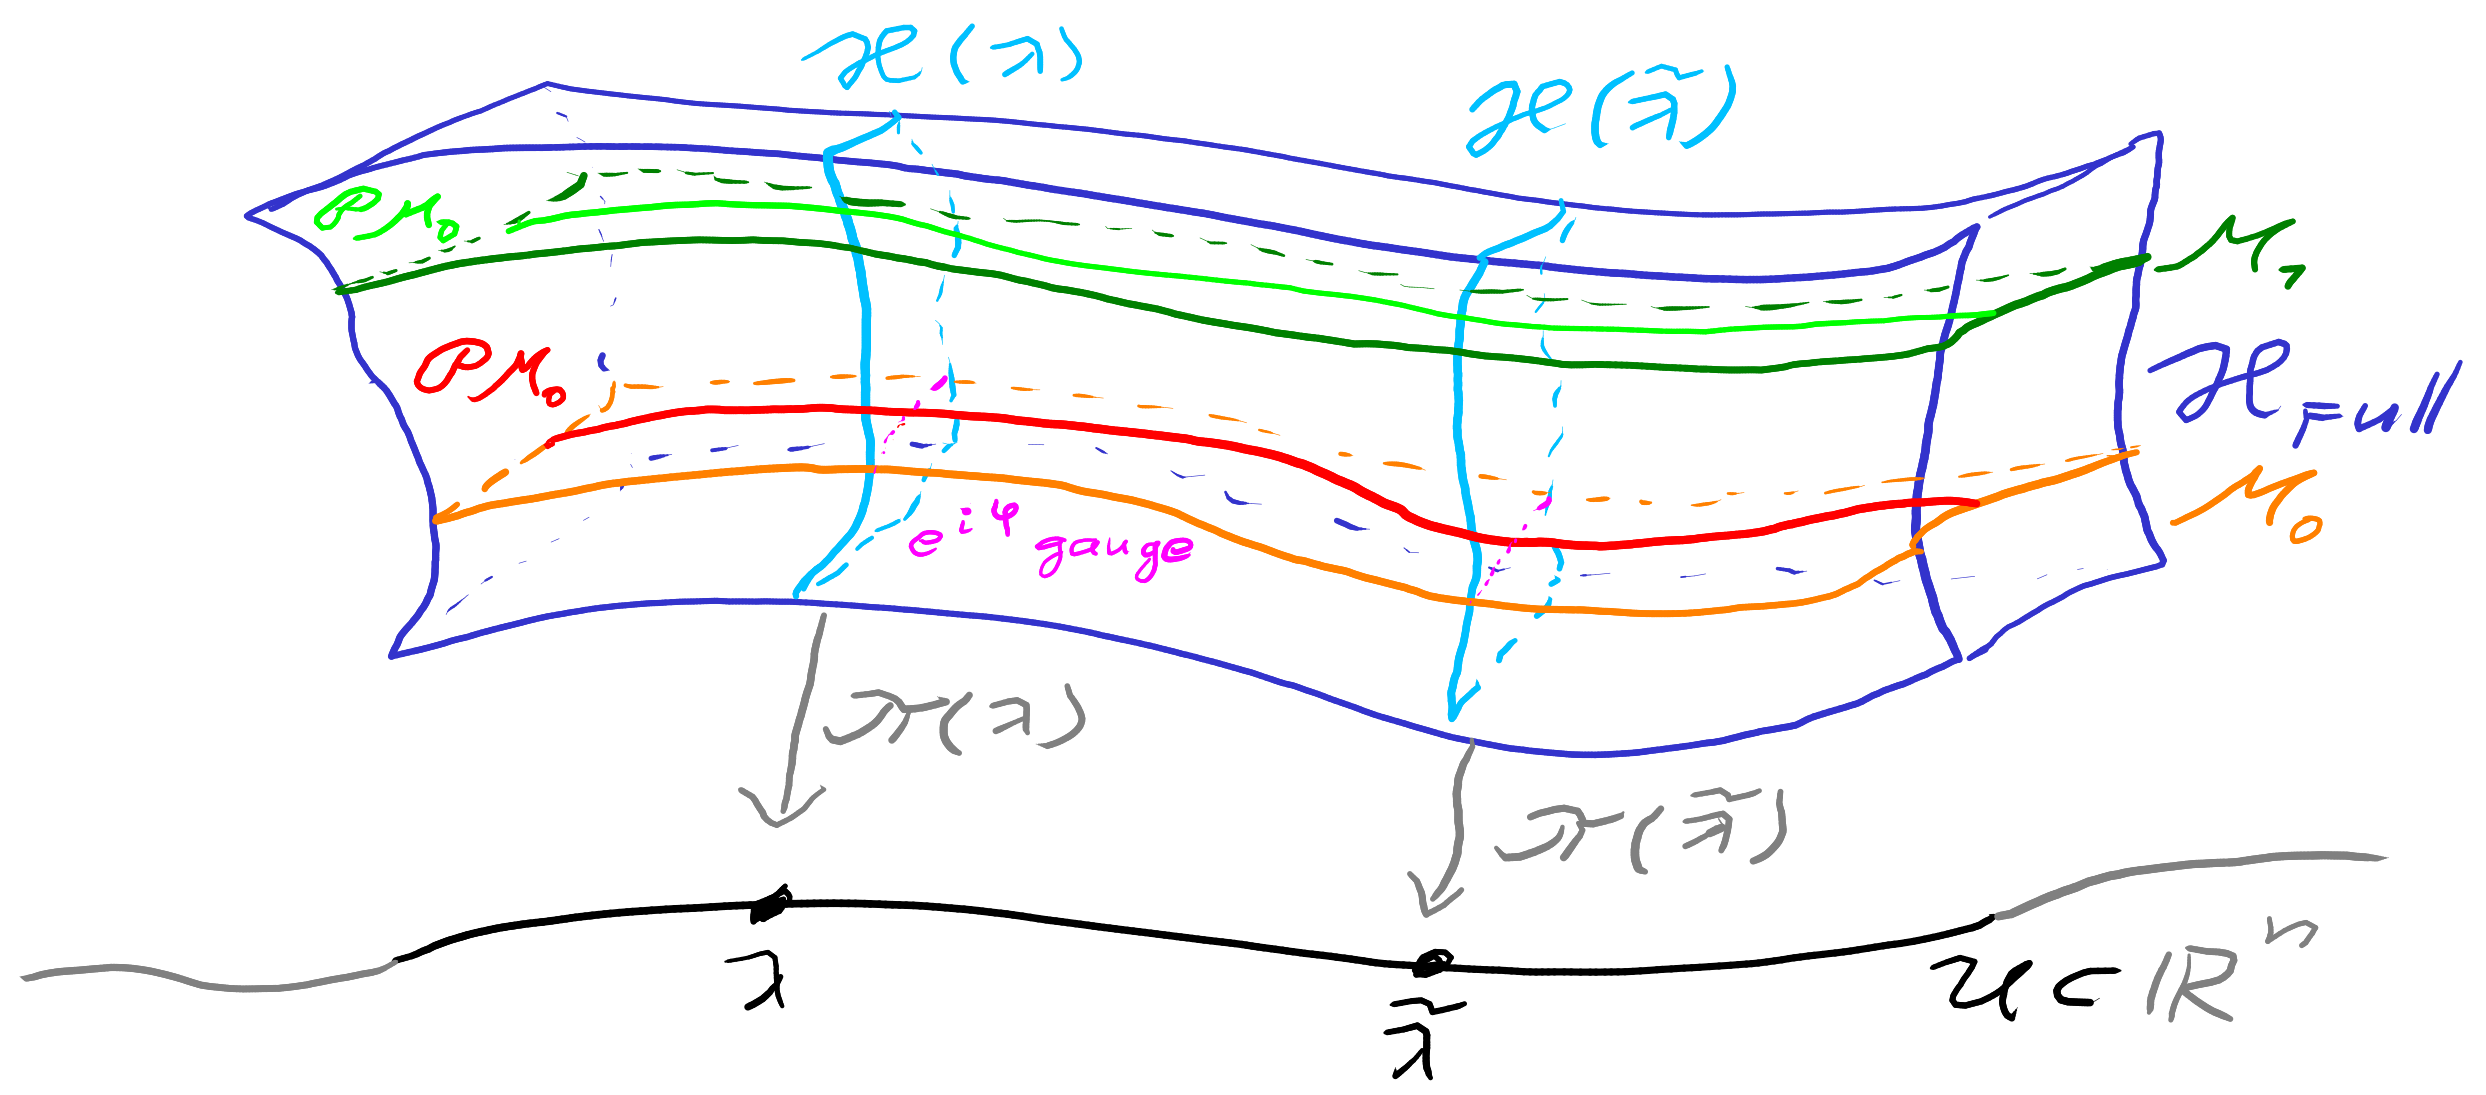
\includegraphics[width=\textwidth]{../img/manifold_full_1.png}
    \begin{tikzpicture}
        \node[] at (0,0) {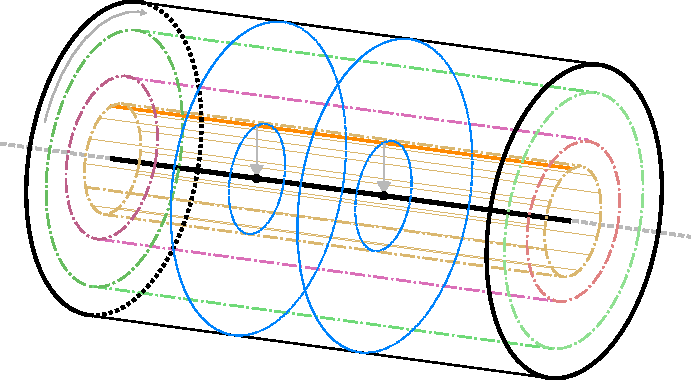
\includegraphics[width=0.7\textwidth]{../img/fullHilbert_1.pdf}};
        \node[] at (5.8,-0.7) {$\mathcal U\subset \gray{\R^N}$};
        \node[] at (4.6,1.8) {$\H_{full}$};
        \node[] at (-1.0,2.7) {$\blueee{\H(\llambda)}$};
        \node[] at (1.0,2.5) {$\blueee{\H(\tilde\llambda)}$};
        \node[] at (-0.8,0.55) {$\gray{\pi(\llambda)}$};
        \node[] at (1.05,0.3) {$\gray{\pi(\tilde\llambda)}$};
        \node[] at (-1.4,-0.17) {$\llambda$};
        \node[] at (0.5,-0.4) {$\tilde\llambda$};
        \node[] at (-3.4,1.43) {$\textcolor{orange}{\P\M_0}$};
        \node[] at (-3.1,1.9) {$\textcolor{magenta}{\P\M_s}$};
        \node[] at (4.0,0.4) {$\textcolor{greenn}{\M_0}$};
        \node[] at (3.8,1) {$\textcolor{violet}{\M_s}$};
        \node[] at (-5.1,2.3) {$\gray{\varphi\in[0,2\pi)}$};
    \end{tikzpicture}
\caption{From the full Hilbert space $\H_{full}$ (the biggest hollow cylinder) we identified eigenstates and unified them into \textcolor{violet}{state manifolds $M_s$}. These are drawn as inner cylinders of $\H_{full}$, especially see the \greenn{ground state manifold $\M_0$} as the \greenn{inner cylinder}. The phase \textcolor{gray}{$\varphi$} introduces gauge symmetry \gray{$e^{i\varphi}$}. If it is fixed, we get projective state manifolds $\textcolor{magenta}{\P\M_s}$, especially see $\textcolor{orange}{\P\M_0}$. Projective state manifolds are isomorphic to the base manifold $\mathcal U$.}
    \label{fig:fullStructure}
\end{figure}




The Hilbert spaces in different points $\llambda$ have the same finite dimension, so the natural question is if we need the fiber structure at all and if we could understand the projection $\pi$ as a surjection from one Hilbert space to the base manifold $\pi: \H\rightarrow \M$. This can indeed be done, but we would lose some generality. For example, the natural choice for basis in the Hilbert space is the eigenbasis, which is different for every $\H(\llambda)$. In addition, dependent on the space structure, two different interpretations of a wave-function collapse can be considered.
\begin{enumerate}
    \item In the fiber structure, we can imagine changing the parameter $\llambda$ as moving between $\H(\llambda)$ subspaces of $\H_{full}$, in which the eigenbasis can be embedded geometrically. The space coordinate then holds information about $\llambda$ and position in Hilbert space. 
    \item If we imagine only one Hilbert space, the eigenbasis varies in time, and the driving is performed in a time-varying space. Therefore, one holds two sets of coordinates — in the Hilbert space and in the parametric space.
\end{enumerate}







\section{Transporting states on state manifolds}
This chapter is inspired by \citet{berry1984}. The decomposition of $\H_{full}$ to different state manifolds $\M_s$ is imagined as sheets above the parametric space. 


Changing the state from eigenstate $\ket{s(\llambda)}$ to $\ket{s(\tilde\llambda)}$ on $\M_s$ during some time period is unitary transformation and can be thought of as \emph{parallel transport on fiber bundle} between two states. Assuming the transport goes along $\mathcal J$ defined by Eq. \ref{eq:defJ}, the transported state can be written at any time as
\begin{equation}
    \hspace{-5pt}\ket{s(\llambda(t))} = \Par_{\gamma_s(t)}\ket{s(\llambda(0))} = \exp\left(-i\int_0^tE_s(\tau)\d\tau)\right)\exp(i\gamma_s(t))\ket{s(\llambda(0))}.
    \label{eq:phasesOnManifold}
\end{equation}


The geometric intuition on driving can be seen on Fig. \ref{fig:manifoldCutIntuition}.
\begin{figure}[H]
    \centering
    % 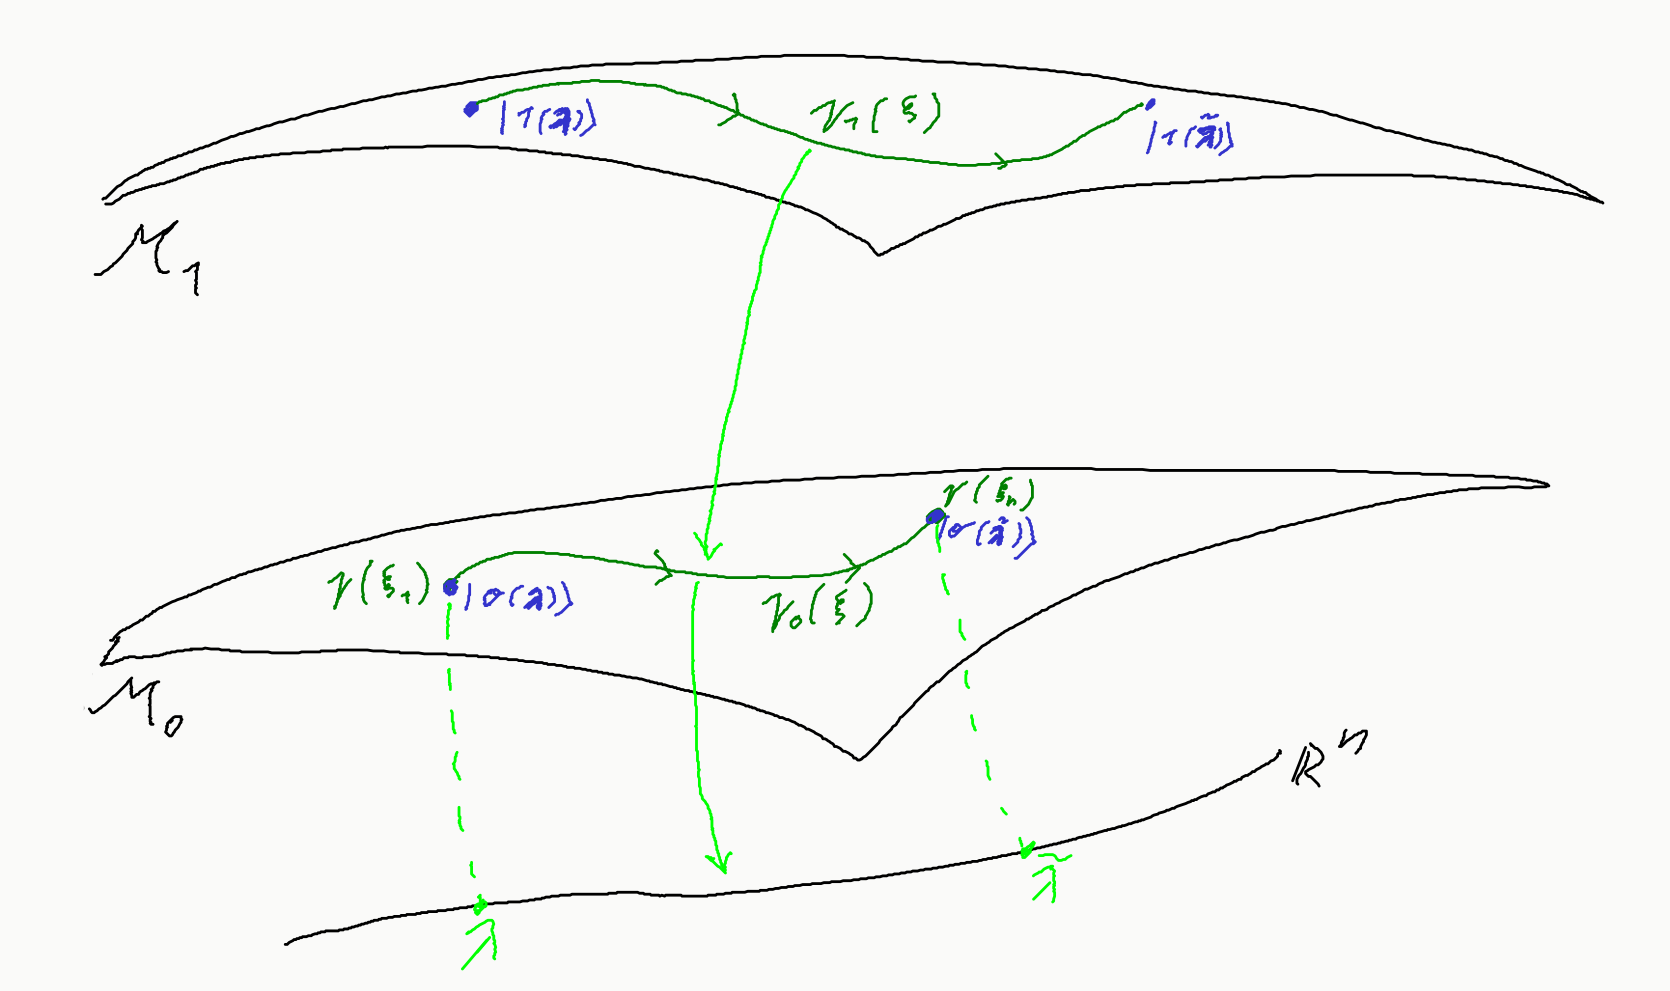
\includegraphics[width=\textwidth]{../img/manifoldCutIntuition.png}
        \begin{tikzpicture}
        \node[] at (0,0) {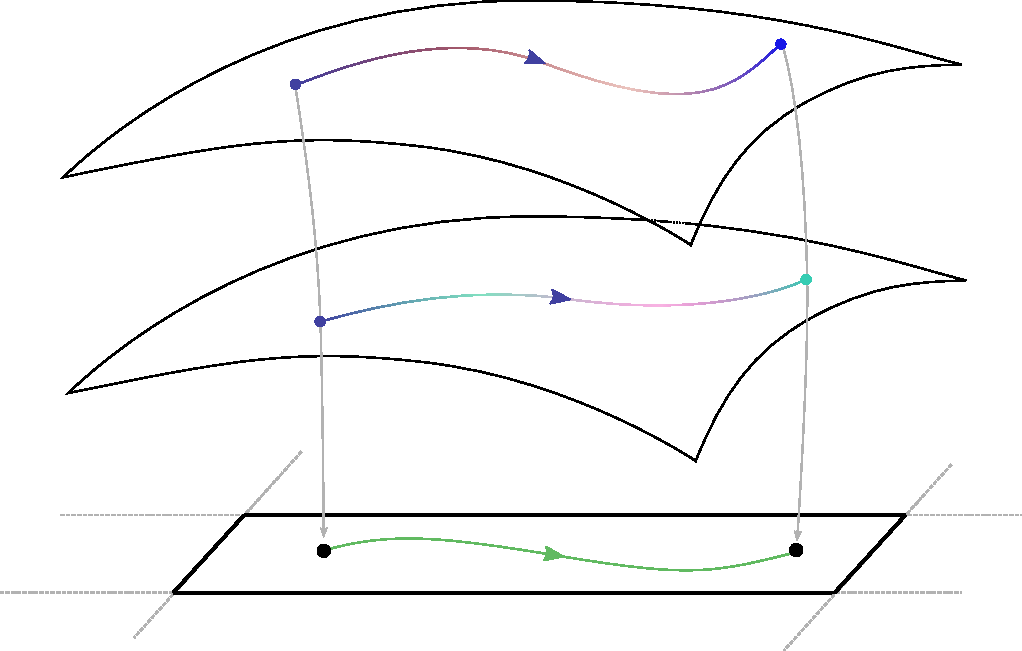
\includegraphics[width=0.9\textwidth]{../img/manifold_structure.pdf}};
        \node[] at (5.1,-3.7) {$\mathcal U\subset \gray{\R^N}$};
        \node[] at (-5.2,-1.1) {$\M_0$};
        \node[] at (-5.2,1.67) {$\M_1$};
        \node[] at (-2.1,2.8) {$\bluee{\ket{1(\llambda)}}$};
        \node[] at (4.2,3.4) {$\blue{\ket{1(\tilde\llambda)}}$};
        \node[] at (-1.8,-0.2) {$\bluee{\ket{o(\llambda)}}$};
        \node[] at (4.4,0.6) {$\greennn{\ket{o(\tilde\llambda)}}$};
        \node[] at (-2.0,-3.1) {$\llambda=\greenn{\mathcal J(0)}$};
        \node[] at (4.7,-2.85) {$\tilde\llambda=\greenn{\mathcal J(T)}$};
        \node[] at (1.2,-2.8) {$\greenn{\mathcal J(t)}$};
        \node[] at (-1.8,-1.8) {$\gray{\pi(\llambda)}$};
        \node[] at (4.3,-1.8) {$\gray{\pi(\tilde \llambda)}$};
    \end{tikzpicture}
\caption{The cylinders from Fig. \ref{fig:fullStructure} are now displayed as two-dimensional sheets. The \bluee{transport of states} is performed on state manifolds $\M_s$ along the \greenn{path $\mathcal J(t)$}, defined in parametric space. The information about gauge phase $\varphi$ is represented by color (see the changing color on the paths in $\M_s$).}
    \label{fig:manifoldCutIntuition}
\end{figure}

Two exponentials in parallel transport in Eq. \ref{eq:phasesOnManifold} have separate meaning and are called \emph{dynamical} and \emph{geometrical} phase.

\subsubsection{Dynamical phase}
The first exponential in Eq. \ref{eq:phasesOnManifold}, the \emph{dynamical phase}, is well known solution to the energy Schr\"odinger equation \ref{eq:energySchrodinger} and depends only on time and Hamiltonian spectrum during the transport. This dynamical phase changes the states only within the projective state manifold $\P\M_s$. 

\subsubsection{Geometrical phase}
The complication arises with the fact that our playground is a state manifold $\M_s$ and some element $\varphi=\gamma_s(t)$, called \emph{geometrical phase}, needs to be included. This phase is generally non-integrable, meaning it depends on the whole path and cannot be written simply as $\gamma_s(\llambda)$. For a closed curve
\begin{equation}
    C=\{\llambda(t)|t\in[0,T] \text{, such that }\llambda(0)=\llambda(T)\}\subset \mathcal U
\end{equation} 
we generally get $\Par_C \ket{\psi(\llambda)}\neq \ket{\psi(\llambda)}$. This property is sometimes called an \emph{anholonomy} and can be imagined on Fig. \ref{fig:manifoldCutIntuition} as change of the path color after circulating around some closed path on $\M_s$. Without anholonomy the path does not change the color. On Fig. \ref{fig:fullStructure}, the change of phase means the curve goes around the inner cylinder $\M_s$ and without anholonomy it gets restricted to $\textcolor{orange}{\P\M_s}$ line.
% and should be defined properly.
% \begin{definition}[Anholonomy]
%     Geometrical phenomenon, which causes some variable $V(\mathcal J(p))$ not to return to it's original value while varying it's parameter $p$ around some closed curve $\mathcal J(p)$. 
% \end{definition}
% and geometric intuition can be seen on Fig. \ref{fig:parallelTransportClosed}. 
% \begin{figure}[h]
%     \centering
%     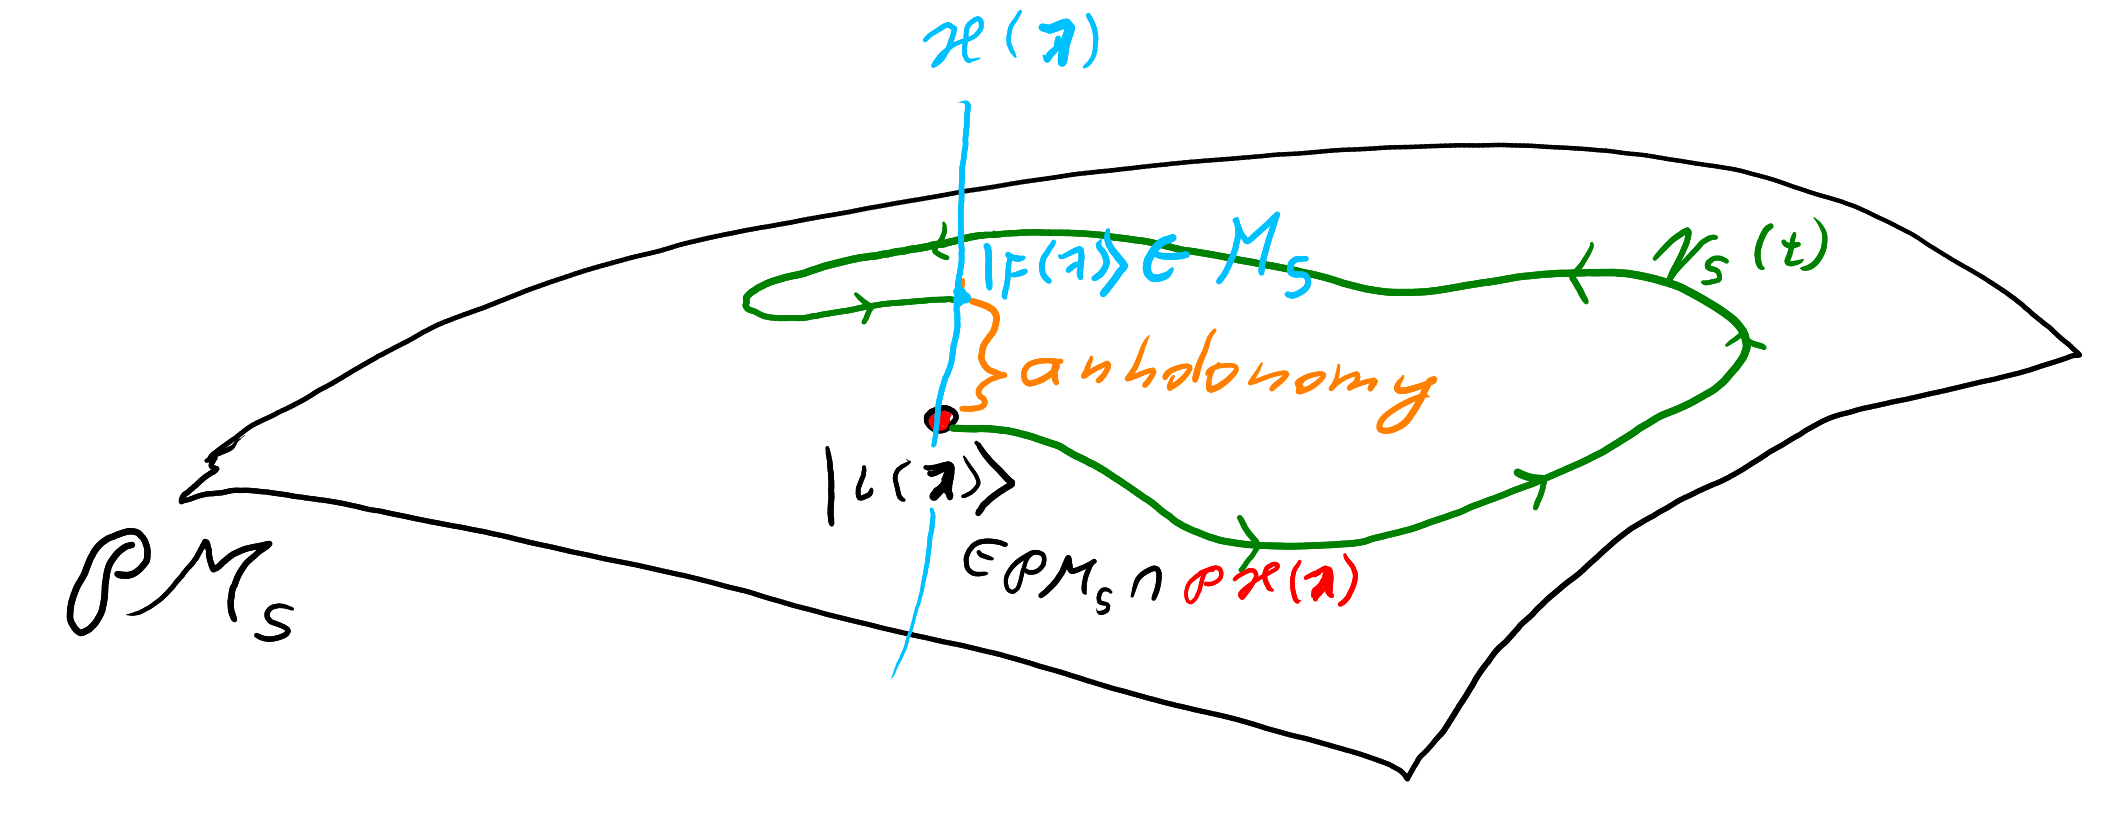
\includegraphics[width=0.8\textwidth]{../img/parallelTransportClosedCurve_1.png}
% \caption{Parallel transport around some \greenn{closed curve $C$}. The \red{eigenstate $\ket{i(\mathcal J(0))}\in\P\M_s$} can be transported to another eigenstate $\ket{f(\mathcal J(T))}\in\M_s$. The \textcolor{orange}{anholonomy} represents their difference in a \blue{gauge} direction.\red{ressemble the pictures above, change the states to $\mathcal J(0),\mathcal J(T)$}}
%     \label{fig:parallelTransportClosed}
% \end{figure}

% For quantum states, the anholonomy can be measured as a non-zero angle between $\ket{V}$ and $\Par_C\ket{V}$, meaning
% \begin{equation}
%     \braket{V|\Par_C|V}\neq 0.
% \end{equation} 


Substituting general solution \ref{eq:phasesOnManifold} to Eq. \ref{eq:schrodinger} yields\footnote{Here the derivation along upper bound $F(x)\coloneqq\int_0^{g(x)}f(t)\d t \Rightarrow F'(x)=f(g(x))g'(x)$ for $f(t)\in L^1(0,g(x))$ and differentiable function $g$, is used.} 
\begin{align}
    \HH(\llambda(t))\kpsit &= i\der{}{t}\kpsit\\
    E_s(\llambda(t)) \ket{s(\llambda(t))} &= E_s(\llambda(t))\ket{s(\llambda(t))} -\der{\gamma_s(t)}{t}\ket{s(\llambda(t))}+ \der{}{t}\ket{s(\llambda(t))}\\
    \der{\gamma_s(t)}{t}&=i\braket{s(\llambda(t))|
    \der{}{t}|s(\llambda(t))}.
\end{align}
 Separating the dependence of vectors on driving parameter and time, we get
\begin{equation}
    \der{\gamma_s(\llambda(t))}{t} =i\braket{s(\llambda(t))|\partial_j s(\llambda)} \dot\llambda^j(\lambda),
\end{equation}
for partial derivative along $\mathcal U$ coordinates $\partial_j$ and dot as time derivative. Integrating this equation around some closed curve $C$ and assuming the dynamical phase to be zero, we get
\begin{equation}
    \gamma_s(C)=i\oint_C\braket{s(\llambda)|\partial_j s(\llambda)}\d \llambda^j.
    \label{eq:gammaCoint}
\end{equation}
This equation implies that the geometric phase does not depend on energy or time, only on the sequence of Hamiltonians, which means it depends only on the path $\mathcal J$ and spectrum $\sigma(\HH(\llambda))$.



\subsubsection{Restriction to 3-dimensional parametric space}
The problem with integration in Eq. \ref{eq:gammaCoint} lies in the derivative $\partial_\llambda s(\llambda)$, which locally requires knowledge of single-valued basis $\{\ket{0},\dots, \ket{N-1}\}$. This can be avoided in 3-dimensions using Stokes's theorem for $S$ as the surface with boundary $\partial S=C$, for coordinate gradient $\bm \nabla$
\begin{equation}
    \begin{split}
        \gamma_s(C) &= -\Im \iint_C \bm\d S \cdot \bm \nabla \times \braket{s(\llambda)|\bm \nabla n(\llambda)}\\
         &= -\Im \iint_C \bm\d S \cdot \braket{\bm \nabla s(\llambda)|\times|\bm \nabla s(\llambda)}\\
        &= -\Im \iint_C \bm\d S \cdot \sum_{m\neq s} \braket{\bm \nabla s(\llambda)|m(\llambda)}\times \braket{m(\llambda)|\bm \nabla s(\llambda)}\\
        &= -\iint_C \bm\d S \cdot \bm V_s(\llambda),
    \end{split}
    \label{eq:stokes}
\end{equation}
for 
\begin{equation}
    \bm V_s(\llambda) = \sum_{m\neq s} \Im \frac{
            \braket{s(\llambda)|\bm \nabla\HH(\llambda) |m(\llambda)}\times \braket{m(\llambda)|\bm \nabla\HH(\llambda)|s(\llambda)}    
             }{
(E_m(\llambda)-E_s(\llambda))^2
             }.
\end{equation}
The element of summation $m=s$ in the third step of derivation \ref{eq:stokes} is real, therefore has no influence on $\gamma_s$ and can be omitted. 

Comparing the first expression in Eq. \ref{eq:stokes} with its last one and extending it to real numbers, we get
\begin{equation}
    \bm V_s(\llambda)=\bm \nabla\times\braket{s(\llambda)|\bm \nabla m(\llambda)}, 
    \label{eq:vectorPotentialDef}  
\end{equation}
defining \emph{vector potential} $\bm V_s(\llambda)$.

\begin{proof}[Proof of Eq. \ref{eq:stokes}]
 All steps are simple algebraic operations, except for the last equivalence. This can be shown by differentiating the Schr\"odinger equation \ref{eq:energySchrodinger}. For any $\ket{s(\llambda)}\in \M_s,\;\ket{m(\llambda)}\in \M_m$ (the dependence on $\llambda$ in notation is omitted), we get
\begin{equation}
    \begin{split}
        \bm \nabla (\overbrace{\HH\ket{s}}^{E_s\ket{s}})&= (\bm\nabla \HH)\ket{\bm \nabla s} +\HH \ket{\bm \nabla s}\\
        \braket{m|E_s|s}&= \braket{m|\bm \nabla \HH| s}+ \underbrace{\bra{m} \HH}_{\bra{m} E_m} |\bm\nabla s\rangle \\
        \braket{m|\bm \nabla s}&=
        \frac{\braket{m|\bm \nabla \HH |s}}
        { E_s-E_m}, \qquad s\neq m,
    \end{split}
    \label{eq:mgradn_proof}
\end{equation}

where $\ket{\bm \nabla s}\coloneqq\bm \nabla \ket{ s}$.    
\end{proof} 

As was mentioned, the above procedure from Eq. \ref{eq:gammaCoint} was performed only for three-dimensional space. Proper generalization to k-dimensional space would yield
\begin{equation}
    \gamma_s(C) = -\iint_C (\bm\d S)^{\alpha\beta} \cdot\Im \frac{
        \overbrace{\braket{s(\llambda)|\bm\d_\alpha \HH(\llambda) |m(\llambda)}}^{\in\TT_1\M}\wedge \overbrace{\braket{m(\llambda)|\bm\d_\beta\HH(\llambda)|s(\llambda)}}^{\in\TT_1\M}    
    }{
        (E_m(\llambda)-E_s(\llambda))^2
    },
    \label{eq:mgrads}
\end{equation}
for exterior derivative $\bm\d$.
                
                
                



\section{Fidelity}
The \emph{fidelity} measures "closeness" of two quantum states. It is generally defined for two density operators $\hat\rho, \hat\sigma$ as
\begin{equation}
    \begin{split}
        \mathcal F&: \End(\H)\times \End(\H)\mapsto \R, \\
        &\mathcal F(\hat\rho,\hat\sigma)\coloneqq \left(\Tr \sqrt{\sqrt{\rho}\sigma\sqrt{\rho}}\right)^2 = \left(\Tr\sqrt[4]{\rho \sigma \sigma \rho}\right)^2= \left(\Tr\sqrt[4]{\rho \sigma (\rho\sigma)^+ }\right)^2,
    \end{split}
    \label{eq:fidelitydef}
\end{equation}
where last equality holds due to hermiticity of density matrices.
The usefulness of this definition can be shown in three special cases.

\begin{itemize}
    \item If both states are pure, $\hat\rho\eqqcolon\ket{\rho}\!\!\bra{\rho}$, $\hat\sigma\eqqcolon\ket{\sigma}\!\!\bra{\sigma}$, the fidelity formula reduces to
    \begin{equation}
        \begin{split}    
            F: \H\times\H&\mapsto \R, \\
            \mathcal F(\hat\rho,\hat\sigma)  \eqqcolon F(\ket{\rho},\ket{\sigma}) &= \left| \braket{\rho|\sigma}\right|^2.
        \end{split}
    \end{equation}

    \item For pure state $\hat\rho=\ket{\rho}\!\!\bra{\rho}$, the fidelity is
    \begin{equation}
        \mathcal F(\hat\rho,\hat\sigma) = \bra{\rho}\hat\sigma \ket{\rho} \left(\Tr\sqrt{\ket{\rho}\!\!\bra{\rho}} \right)^2 = \bra{\rho}\hat\sigma \ket{\rho}.
    \end{equation}
    
    \item Commuting density matrices have a meaning of probability distributions. The commutativity implies that $\hat\rho,\hat\sigma$ can be diagonalized in the same eigenbasis. For $\hat\rho = \sum_i p_i \ket{i}\!\!\bra{i}$, $\hat\sigma = \sum_i s_i \ket{i}\!\!\bra{i}$ we get
    \begin{equation}
        \sqrt{\hat\rho \hat\sigma}=\Tr\left(\sum_k\sqrt{p_k s_k}\ket{i}\!\!\bra{i}\right)=\sum_k\sqrt{p_k s_k}
    \end{equation}
    and inserting into the definition \ref{eq:fidelitydef} gives
    \begin{equation}
        F(\hat\rho,\hat\sigma)=\left(\sum_k\sqrt{p_k s_k}\right)^2.
    \end{equation} 

\end{itemize}
    
    
The physical meaning of fidelity can also be seen on the state manifolds, imagining \emph{quantum quench between two states} (rapid change of some Hamiltonian parameters). In this case, $F$ is the probability that the system prepared in some initial ground state $\ket{\rho}$ is found in the new ground state $\ket{\sigma}$. $1-F$ is then the probability of exciting the system during this quench.

Before moving to the practical usage of fidelity, let's look at some general properties.
    

\begin{thm}[The fidelity properties]
    For any two density matrices $\hat\rho,\;\hat\sigma$
    \begin{itemize}
        \item $\mathcal F(\hat\rho,\hat\sigma)\in[0,1]$ \emph(normalization\emph),
        \item $\mathcal F(\hat\rho,\hat\sigma) = \mathcal F(\hat\sigma,\hat\rho)$ \emph(symmetry\emph),
        \item $\mathcal F(\hat\rho,\hat\sigma)=1 \Leftrightarrow \hat\rho=\hat\sigma$.
    \end{itemize}
\end{thm}
\begin{proof}
    The first statement is a consequence of Cauchy-Schwarz inequality. The second and third go from Uhlmann's theorem, see publication from \citet{uhlman}.
\end{proof}



\section{Metric and geometric tensor}
\label{chap:metricTensor}
As a playground for this chapter, we choose the projective ground state manifold $\P\M_0$, but it can be easily generalized to any $\P\M_s$. This means the geometrical phase is neglected, because the states are considered to be the physical states from the projective Hilbert space.
% Our first guess might be
% \begin{equation}
%     \d \tilde{s}^2 = \braket{i(\bm\llambda+\d\bm\llambda)|i(\bm\llambda+\d\bm\llambda)} = 1-2\Re{\braket{i(\bm\llambda+\bm\d\llambda)|i(\bm\llambda)}}.
% \end{equation}
% This is \emph{gauge dependent}, meaning that it depends on our choice of the wave phase, i.e. on observer. 

To obtain restriction on metric tensor definition, the local gauge dependence needs to be suppressed. This means the distance on $\P\M_0$ cannot depend on coordinate dependent gauge phase $\varphi(\llambda)$. This phase induces the change in a ground state $\ket{o(\llambda)}$ of the Hamiltonian $\HH(\llambda)$\footnote{Note that we can also write $\ket{o(\llambda)}\in \P\M_0\cap \H(\llambda)$, which is the set containing exactly one vector -- the ground state of $\HH(\llambda)$.}
\begin{equation}
    \ket{o(\llambda)}\mapsto e^{i\varphi(\llambda)} \ket{o(\llambda)},
\end{equation}
which implies
\begin{equation}
        \braket{o(\llambda)|\bm \nabla o(\llambda)}\mapsto \braket{o(\llambda)|\bm \nabla o(\llambda)} + i\bm \nabla \varphi(\llambda) 
\end{equation} 
For twice differentiable function $\varphi(\llambda)\in \mathcal C^2$, the gauge independent function $f$ would be for infinitesimal change for example
\begin{equation}
    f\coloneqq \braket{o(\bm\llambda+\delta\bm\llambda)|o(\bm\llambda)},
    \label{eq:fidelityDefinition}
\end{equation}
sometimes referred to as the \emph{fidelity amplitude of a ground state}, because for pure states we get the fidelity $F=|f|^2$. The meaning of fidelity as a probability transition between the states during some quench, leads to the definition of \emph{distance on $\M_0$}
\begin{equation}
    \d s^2 \equiv 1-F(\ket{o(\bm\llambda+\delta\bm\llambda)},\ket{o(\llambda)})= 1-\left|\braket{o(\bm\llambda+\delta\bm\llambda)|o(\bm\llambda)}\right|^2.
    \label{eq:distanceOnM0}
\end{equation}
We can easily check, that the axioms for metric distance holds:
\begin{itemize}
    \item identity of indiscernibles $s(\kpsi,e^{i\alpha}\kphi) = 0 \Leftrightarrow \kpsi=\kphi$, $\alpha\in\R$,
    \item symmetry for any two states $\kpsi$, $\kphi$ is implied by $|\braket{\psi|\varphi}|=|\braket{\varphi|\psi}|$,
    \item triangle inequality: $s(\kpsi,\ket{\psi_2}) <s(\kpsi,\ket{\psi_1}) + s(\ket{\psi_1},\ket{\psi_2})$\\
    for any $\ket{\psi}$,$\ket{\psi_1}$,$\ket{\psi_2}$.
\end{itemize}
If we take the fidelity between two parameter-dependent states, the infidelity $1-F(\ket{\psi(\llambda)},\ket{\psi(\llambda+\Delta)})>0$ and the first term of Taylor expansion in $\Delta$ is zero, implying it can be used for the metric tensor definition.

\begin{definition}[Metric tensor on projective state manifolds]
    \label{def:metricTensor}

Because the projective state manifolds $\P\M_s$ are isomorphic to the base manifold $\R^N$, we can define
    \begin{equation}
        \begin{split}
            g_{\mu\nu}&: \redd{\T\mathcal U}\times \redd{\T\mathcal U}\rightarrow \R \\
            g_{jk}\redd{\d \bm \lambda^j \d\bm \lambda^k}+\O(\lambda^3) \equiv \d s^2 &\coloneqq 1-\left|\braket{o(\bm\llambda+\delta\bm\llambda)|o(\bm\llambda)}\right|^2.
            \label{eq:metricTensorDef}
        \end{split}
    \end{equation} 
   
\end{definition}
Even though we call $g_{\mu\nu}$ the metric tensor \emph{on projective state manifolds}, it takes forms from $\redd{\T\mathcal U}$. Using abstract indices this means
\begin{equation}
    g^{\mu\nu}\redd{\d_\mu \llambda \d_\nu \llambda}.
\end{equation}
This whole procedure can be made more rigorous using so-called \emph{vector bundles}, see the book by \citet{lu}[Chap. 7]. In our case we can use the isomorphism of $\redd{\T\mathcal U}\times \redd{\T\mathcal U}$ and $\bluee{\T\M}\times \bluee{\T\M}$ and simply write
\begin{equation}
    g_{jk}\redd{\d\llambda^j \d\llambda^k} = g_{jk}\frac{\redd{\partial\llambda^j}}{\bluee{\partial\bm v^l}}\frac{\redd{\partial\llambda^k}}{\bluee{\partial\bm v^m}} \bluee{\d\bm v^l \d \bm v^m} \eqqcolon G_{lm}\bluee{\d\bm v^l \d \bm v^m}.
\end{equation}
Practically only $g_{jk}$ is used; thus, what should have been called \emph{the metric tensor on state manifolds} $G_{\mu\nu}$ leaves forgotten. "And some things that should not have been forgotten were lost." \citet{lordOfTheRings}







% \subsubsection{Geometric tensor}
% \red{Add more info from quantum\_geometric\_tensor\_pedagogical.pdf The scalar product (braket) of two quantum states is a 2-form $\chi_{\mu\nu}: \H\times\H\rightarrow \C$ and can be decomposed to real and imaginary part as
% \begin{equation}
%     \braket{\psi_1|\psi_2}\equiv \chi(\psi_1,\psi_2)=g(\psi_1,\psi_2)-i\nu(\psi_1,\psi_2).
%     \label{eq:quantumProd}
% \end{equation}
% }
% \red{From braket sesquilinearity goes that $g_{\mu\nu}$ is symmetric and $\nu_{\mu\nu}$ antisymmetric, thus they can be uniquely written into one 2-form $\chi_{\mu\nu}$, called the \emph{Fubini-Study metric} or the \emph{Geometric tensor}, with property
% \begin{equation}
%     g=\Re \chi ;\qquad \nu=\Im \chi.
% \end{equation}
% Here we call the $g$ a \emph{metric tensor} and $k$ the \emph{curvature tensor}, or \emph{Berry curvature}. 
% }
% The distance between quantum states can also be defined as
% \begin{equation}
%     \d s^2 \coloneqq |\psi(\llambda+\d \llambda)-\psi(\llambda)|^2 = \braket{\delta\psi|\delta\psi} = \underbrace{\braket{\partial_j\psi|\partial_k\psi}}_{\chi_{jk}(\llambda)} \d\llambda^j \d\llambda^k 
% \end{equation}

Because the metric tensor is a real analytical function of coordinates, its analytical continuation into complex numbers can be performed. For the motivation behind the following definition, see the book by \citet{cheng_quantum_2013}.

\begin{definition}[Geometric tensor]
    On the ground state manifold $\M_0$, the geometric tensor can be defined as
    \begin{equation}
        \chi_{jk}\coloneqq \braket{\partial_j o|\partial_k o}_c \equiv \braket{\partial_j o|\partial_k o} - \braket{\partial_j o|o}\braket{o|\partial_k o},
        \label{eq:geometricTensor}
    \end{equation}
    where shortened notation $\partial_k\coloneqq\pder{}{\llambda^k}$ is used. The subscript $c$ means \emph{connected} and is defined by the formula.
\end{definition}
This definition is in fact gauge independent and can be extended onto any state manifold. 

Real part of geometric tensor is symmetric, and it is the metric tensor from Def. \ref{def:metricTensor}. The imaginary part is antisymmetric and is called the \emph{curvature tensor}, or \emph{Berry curvature}. The metric tensor can then be expressed as
\begin{equation}
    g_{jk} =\Re \chi = \frac{1}{2}(\chi_{jk}+\chi_{kj}) = \Re \sum_{o\neq s}\frac{\braket{o|\pder{\H}{\llambda^j}|s}\braket{s|\pder{\H}{\llambda^k}|o}}{(E_o-E_s)^2}.
    % =\Re\braket{\partial_j o|\partial_k o}_c = 
    \label{eq:metrictensorREdefinition}
\end{equation}
The Berry curvature is
\begin{equation}
        \nu_{jk} =\Im \chi= \frac{i}{2}(\chi_{jk}-\chi_{kj})=  - \Im \sum_{o\neq s}\frac{\braket{o|\pder{\H}{\llambda^j}|s}\braket{s|\pder{\H}{\llambda^k}|o}}{(E_o-E_s)^2}.
        % =\frac{1}{2}\Im\braket{o|[\curlyleftarrow{\partial}_k,\partial_j]|o}_c =
    \label{eq:geom.tensorREdefinition}
\end{equation}

%taylor is wrong
% \begin{proof}[Proof for Geometric tensor expression] In one-dimensional case we get from eq. \ref{eq:fidelityDefinition} using Taylor expansion and shortened notation $o\coloneqq o(\llambda)$
%     \begin{equation}
%         f=1+\braket{\partial_\llambda o|o}\delta\llambda-\frac{1}{2}\braket{\partial_\llambda^2 o|o}\delta\llambda^2+\mathcal{O}(\llambda^3),
%     \end{equation}
%     which plugged into eq. \ref{eq:distanceOnM0} gives
%     \begin{equation}
%         \begin{split}
%             \d s^2&=1-\bar{f}f=\left[-\braket{o|\partial_\llambda o}\braket{\partial_\llambda o|o}+\frac{1}{2}\braket{\partial_\llambda^2 o|o}+\frac{1}{2}\braket{o|\partial_\llambda^2 o}\right]\delta \llambda^2.
%         \end{split}
%     \end{equation}
%     Generalizing for $\llambda\in \R^N$, we get\footnote{assuming Hermiticity of the derivative operator everywhere on the ground state manifold}
%     \begin{equation}
%         \d s^2=\left[-\braket{o|\partial_j o}\braket{\partial_k o|o}+\underbrace{\frac{1}{2}\braket{o|\partial_j \partial_k|o}+\frac{1}{2}\braket{o|\partial_k \partial_j| o}}_{\Re\braket{\partial_mu o|\partial_k o}}\right]\delta \llambda^j\delta \llambda^k.
%     \end{equation}
%     Because only symmetric part contributes in the sum in eq. \ref{eq:metricTensorDef}, this proves symmetric part of equation \ref{eq:geometricTensor} and shows, that some more general tensor (\emph{geometric tensor}) exists.
% \end{proof}



\begin{proof}[Proof of the  metric tensor definitions correspondence]\
    \label{sec:derivationOfGeometricTensor}

    To prove the correspondence of geometric tensor, defined by Eq. \ref{eq:geometricTensor}, to distance on $\M_0$ in Eq. \ref{eq:distanceOnM0}, we start with the state $\ket{o(\llambda)}\in \M_s\cap\H(\llambda)$ — the ground state of $\HH(\llambda)$. Changing parameter $\llambda$ to $\llambda+\delta \llambda$ results in a state, which is a linear combination of eigenstates $\ket{s(\llambda+\delta \llambda)}\in \M_s\cap\H(\llambda+\delta \llambda)$, meaning the state is no longer eigenstate. Its collapse to any new eigenstate has a probability amplitude
    \begin{equation}
        \begin{split}
            a_s&=\braket{s(\llambda+\delta\llambda)|o(\llambda)}\approx \delta\llambda^j\braket{\partial_j s(\llambda)|o(\llambda)} \\
            &= -\delta\llambda^j\braket{s(\llambda)|\partial_j|o(\llambda)}.
        \end{split}
    \end{equation}

    If we introduce the \emph{gauge potential}, sometimes called the \emph {calibration potential}, as\footnote{In SI units, the gauge potential is $\AA_j\coloneqq i\hbar\partial_{j}$}
    \begin{equation}
        \AA_j\coloneqq i\partial_{j},
    \end{equation}
    the probability amplitude can be expressed as
    \begin{equation}
    a=i\braket{s(\llambda)|\AA_j |o(\llambda)}\delta\llambda^j,
    \label{eq:probabilityOfTransitionIsGauge}
    \end{equation}
    which has a meaning of gauge potential matrix elements. Probability of the excitation, i.e. the transition to any state $s>0$ from ground state is then (omitting the $\llambda$ dependence in notation)
    \begin{equation}
        \begin{split}
            \sum_{s\neq 0}|a_s|^2&=  \sum_{s\neq 0} \delta \llambda^j \delta \llambda^k\bluee{\braket{o|\AA_j|s}\braket{s|\AA_k|o}}\gray{+\O(|\delta \llambda^3|)} \\
            &= \delta \llambda^j \delta \llambda^k\bluee{\braket{o|\AA_j \AA_k|o}_c}\gray{+\O(|\delta \llambda^3|)}\eqqcolon \delta \llambda^j \delta \llambda^k\bluee{\chi_{jk}}\gray{+\O(|\delta \llambda^3|)},
        \end{split}
    \end{equation}
    where last term defines the \bluee{geometric tensor}.
\end{proof}






The calibration invariance of the gauge potential can be explained using the Berry connection.
\begin{definition}[Berry connection]    
    On the ground state manifold $\M_0$, the \emph{Berry connection} is defined as the mean value of gauge potential
    \begin{equation}
        A_j(\llambda)\coloneqq \braket{o(\llambda)|\AA_j|o(\llambda)}= -i \braket{o(\llambda)|\partial_j|o(\llambda)}.
        \label{eq:berryConnection}
    \end{equation}
\end{definition}
    

This empowers us to take derivatives in any direction and the expression for geometric tensor on $\M_0$
\begin{equation}
    \chi_{jk}(\llambda) = \partial_j A_k(\llambda)-\partial_k A_j(\llambda)
    \label{eq:geometricTensorRedef}.
\end{equation}
This formula can be directly proven by comparing with \ref{eq:geometricTensor}. Here we see that the calibration invariance is 
\begin{equation}
    A_j \mapsto A_j+\partial_j \alpha(\llambda),\qquad \alpha\in\mathcal C^2,
\end{equation}
meaning any twice differentiable function can be added to the gauge potential, leaving the geometric tensor unchanged.

\begin{definition}[Berry phase]
    
    The \emph{Berry phase}, as an integral of the Berry connection along some closed curve $\mathcal{C}$\footnote{
        The reasonability of this definition can be seen, if we assume the ground state of a free particle
        $\braket{\bm{x}|i(\llambda)}\equiv i(\bm{x},\llambda)= |i(\bm{x})|e^{i\phi(\llambda)}$,
        then the Berry connection is
        \begin{equation}
            A_j=-\int \d \bm{x}|i(\bm{x},\llambda)|^2\partial_j \phi(\llambda) = -\partial_j \phi(\llambda)
        \end{equation} 
        and Berry phase
        \begin{equation}
            \varphi_B=\oint_\mathcal{C} \partial_j \phi \d \llambda^j,
        \end{equation}
        which represents total phase accumulated by the wave function. It is really the analogy for Berry phase in classical mechanics, which for example in the case Foucault pendulum on one trip around the Sun makes $\varphi_B=2\pi$
        }

    \begin{equation}
        \varphi_B\coloneqq-\oint_\mathcal{C} A_j(\llambda)\d \llambda^j=\int_\mathcal{S} \chi_{jk}(\llambda)\d \llambda^j \wedge \d\llambda^k,
    \end{equation}
    where we used the Stokes theorem for some area $\mathcal{S}$ with boundary $\partial\mathcal{S}=\mathcal{C}$.    
    
\end{definition}

Berry phase is zero when the curve does not go around some geometric tensor singularity. The number of \emph{how many times the curve goes counterclockwise around some point of interest} is defined as \emph{winding number} $\mathrm{Ind}$. In this case, the points of interest are singularities $a$, and
$$\mathrm{Ind}_a \mathcal J(\llambda)=0 \Rightarrow \varphi_B=0.$$

In the case of the ground-state manifold, these singularities appear in the system due to energy spectrum degeneracies when $E_1-E_0=0$. These points are called \emph{diabolic} because of the energy spectrum shape in the parametric space.\footnote{https://en.wikipedia.org/wiki/Diabolo}